% Compile with pdfLaTeX.
% Landscape version corresponding to the revised portrait template.
% Font matching is intentionally relaxed for this version.

\documentclass[a4paper,landscape]{article}

% Scroll down to line 74

% Minimal external packages:
\usepackage[a4paper,landscape,left=18mm,right=18mm,top=18mm,bottom=18mm]{geometry}
\usepackage{graphicx}
\usepackage{xcolor}
\usepackage{lipsum}
\usepackage{array}
\usepackage[T1]{fontenc}
\usepackage[sfdefault]{roboto}
\usepackage[
    colorlinks=true,
    urlcolor=blue,
    linkcolor=black,
    citecolor=blue
]{hyperref}

\pagestyle{empty}
\setlength{\parindent}{0pt}
\setlength{\parskip}{0pt}
\setlength{\tabcolsep}{0pt}
\definecolor{topicblue}{HTML}{2F5597}

% Lengths - specifications for template fonts, appearance
\newlength{\HeaderSize}
\setlength{\HeaderSize}{24pt}
\newlength{\HeaderSizeBaseline}
\setlength{\HeaderSizeBaseline}{28.8pt}

\newlength{\SectionSize}
\setlength{\SectionSize}{16pt}
\newlength{\SectionSizeBaseline}
\setlength{\SectionSizeBaseline}{1.2\SectionSize}

\newlength{\TextSize}
\setlength{\TextSize}{14pt}
\newlength{\TextSizeBaseline}
\setlength{\TextSizeBaseline}{1.3\TextSize}

\newlength{\CaptionSize}
\setlength{\CaptionSize}{12pt}
\newlength{\CaptionSizeBaseline}
\setlength{\CaptionSizeBaseline}{1.2\CaptionSize}

\newlength{\RefSize}
\setlength{\RefSize}{12pt}
\newlength{\RefSizeBaseline}
\setlength{\RefSizeBaseline}{1.4\RefSize}

\newlength{\vskipHeader}
\setlength{\vskipHeader}{8.0mm}
\newlength{\vskipSection}
\setlength{\vskipSection}{4.0mm}
\newlength{\vskipText}
\setlength{\vskipText}{2.0mm}
\newlength{\vskipImage}
\setlength{\vskipImage}{16.0mm}

% Landscape geometry.
% The left panel is square; the right panel uses the remaining width.
\newlength{\LeftPanel}
\setlength{\LeftPanel}{164mm}
\newlength{\PanelGap}
\setlength{\PanelGap}{18mm}
\newlength{\RightPanel}
\setlength{\RightPanel}{79mm}

% Do not change anything above this line!

\begin{document}
\noindent
\begin{tabular}{@{}p{\LeftPanel}@{\hspace{\PanelGap}}p{\RightPanel}@{}}

% ======================= LEFT SQUARE =======================
\parbox[t][\LeftPanel][t]{\LeftPanel}{%

% High page header
\begin{center}
  {\fontsize{\HeaderSize}{\HeaderSizeBaseline}\selectfont\color{topicblue}%
  %
  % Agnese will modify this; For now write your name and number your projects with 1 and 2
   Project Topic:\hspace{9mm} (Agnese 1)} 
\end{center}

\vspace{\vskipHeader}

% Main title
{\fontsize{\SectionSize}{\SectionSizeBaseline}\selectfont\bfseries 
%
% Title
Nature-inspired patterns
\par}
\vspace{\vskipSection}

% Abstract / project description --> adjust accordingly
{\fontsize{\TextSize}{\TextSizeBaseline}\selectfont
%
% Intro+Motivation
Nature is a rich source of inspiration for the study and design of complex systems. Animals, even seemingly simple organisms, are capable of building remarkable structures and interacting with each other through complex collective behaviors. Such natural patterns have often inspired engineering solutions, computational methods, and models of social organization.
\par

\vspace{\vskipText}
% In this project
In this project, you will identify a nature-inspired complex pattern and develop a simulation to reproduce and investigate it. For example, how can the construction of a spider web be modeled? How does the collective behavior of an ant colony emerge from simple individual rules? The goal is to explore how relatively simple mechanisms and interactions can give rise to complex structures or behaviors, and to assess how effectively they can be captured through simulation.
\par
}

\vfill

% References are entered manually. No .bib file / BibTeX / biblatex.
{\fontsize{\SectionSize}{\SectionSizeBaseline}\selectfont\bfseries References:\par}
\vspace{\vskipSection}

{\fontsize{\RefSize}{\RefSizeBaseline}\selectfont
% 
% Reference 1
[1] Aoyanagi, Y. and Okumura, K. \textit{Simple Model for the Mechanics of Spider Webs}, Phys. Rev. Lett. \textbf{104}, 038102 (2018).\\
\href{https://journals.aps.org/prl/abstract/10.1103/PhysRevLett.104.038102}{https://journals.aps.org/prl/abstract/10.1103/PhysRevLett.104.038102} 
\par
% 
% Reference 2 (if needed)
[2] Freas, C.A., Buehlmann, C. \& Spetch, M.L. \textit{Combining social and private information: How ants use pheromones and learnt cues to navigate}. Learn. Behav. \textbf{54}, 23–36 (2026). \\
\href{https://link.springer.com/article/10.3758/s13420-025-00697-w}{https://link.springer.com/article/10.3758/s13420-025-00697-w}
\par
% 
% Add a Reference 3 (if needed)
}
\vspace{\vskipText}
}% end left square

&

% ======================= RIGHT COLUMN =======================
\parbox[t][\LeftPanel][c]{\RightPanel}{%
\centering
%
% Representative image + caption. 
\begin{tabular}{@{}c@{}}
%
% Image
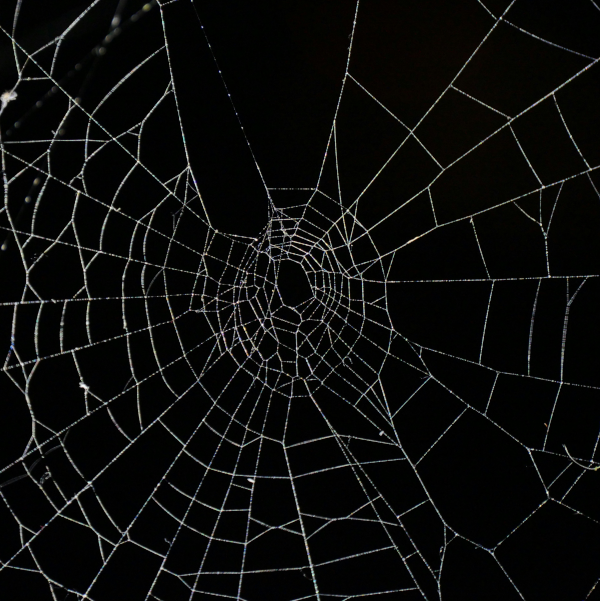
\includegraphics[width=\RightPanel]{spiderweb.png}\\[\vskipSection] % name of the image 
\parbox{\RightPanel}{%
\fontsize{\CaptionSize}{\CaptionSizeBaseline}\selectfont
\textbf{Fig.1}\quad 
% 
% Title of the image (bold)
\textbf{Photo of a spider web.} 
% 
% Body of the image caption.
Spider webs are remarkable natural architectures for capturing prey. Vibrations propagating through the silk allow the spider to detect and locate captured prey, providing an elegant example of how complex functionality can emerge from structure and material properties.
%
% Credits.
\textit{Photo by Rafael Garcin on \href{https://unsplash.com/photos/spider-web-in-close-up-photography-wlOv3cf41iE}{Unsplash}} 
}
\end{tabular}
}% end right column

\end{tabular}
\end{document}
